\subsection{Borrow Checker}
\label{sec:BorrowCheckerDesign}

The \borrowChecker{} implements the visitor pattern (see
section~\ref{sec:VisitorDesign}) and uses this to traverse the \ast{} in a depth
first, left to right pattern. It uses two tables a \texttt{symbolTable} and a
\texttt{referenceTable} to keep track of the scopes and the
references of each variable.

\begin{lstlisting}[
  frame=single,
  numbers=left,
  label={lst:BorrowCheckerCode},
  caption={Example Program to illustrate how the \borrowChecker{} is designed   to walk the \ast{} and use tables to keep track of references},
  ]
  fn main(): int {
    let mut x: int = 1;
    let y: &int = &mut x; // declaration of mutable reference
    let z: &int = &x; // declaration of immutable reference
    return 0;
  }
\end{lstlisting}

Consider the example program (see Listing~\ref{lst:BorrowCheckerCode}) and the
accomanying subtree (see Figure~\ref{fig:astBorrowCheckerDesignCode}). The
\borrowChecker{} visits each node
in a depth first order and at each point it determines based on the \texttt{symbolTable}
and the \texttt{referenceTable} if the
program is in compliance with the ownership, borrowing and reference rules (see
section~\ref{par:Ownership}).

\begin{figure}[ht]
  \centering
  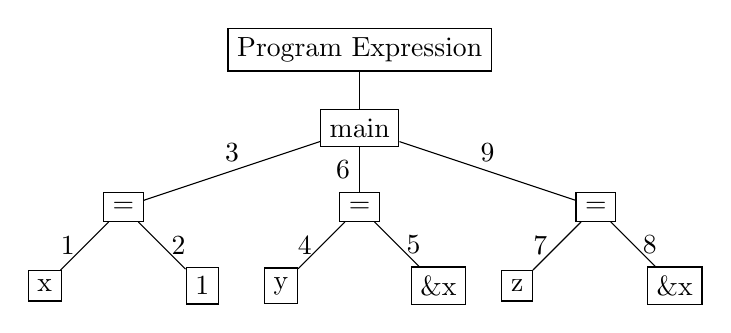
\begin{tikzpicture}

    \node[draw] (program) at (0,0){Program Expression};

    \node[draw] (main) at (0,-1){main};

    \node[draw] (assign) at (-3, -2){=};
    \node[draw] (x) at (-4, -3){x};
    \node[draw] (term) at (-2, -3){1};

    \draw[] (program) -- (main);
    \draw[] (main) -- node[above]{3} (assign);
    \draw[] (assign) -- node[left]{1} (x);
    \draw[] (assign) -- node[right]{2} (term);

    \node[draw] (assign2) at (0, -2){=};
    \node[draw] (y) at (-1, -3){y};
    \node[draw] (ref) at (1, -3){\&x};

    \draw[] (main) -- node[left]{6} (assign2);
    \draw[] (assign2) -- node[left]{4} (y);
    \draw[] (assign2) -- node[right]{5} (ref);

    \node[draw] (assign3) at (3, -2){=};
    \node[draw] (z) at (2, -3){z};
    \node[draw] (ref2) at (4, -3){\&x};

    \draw[] (main) -- node[above]{9} (assign3);
    \draw[] (assign3) -- node[left]{7} (z);
    \draw[] (assign3) -- node[right]{8} (ref2);

  \end{tikzpicture}
  \caption{Program \ast{} ignoring the return statement. The numbering showing the
  order that the \borrowChecker{} proccess each node.}
  \label{fig:astBorrowCheckerDesignCode}
\end{figure}

In the example program, the \borrowChecker{} will add the \texttt{x} variable to the
\texttt{symbolTable}. When it creates a reference to \texttt{x}, it will look up
\texttt{x} to ensure it is an existing variable that can be referenced, then it will
store \texttt{y} in the \texttt{symbolTable} as well as a reference in the
\texttt{referenceTable} to determine if future references are legal to perform. 

Once it reaches the last instruction, it will look up \texttt{x} in the
\texttt{symbolTable}, which is fine, but it will determine from the
\texttt{referenceTable} that a mutable reference already exists. Thus the last
instruction is an illegal operation as immutable and mutable references cannot exist
at the same time (see Section~\ref{par:Ownership}). The compiler will then inform the
user that the program is not a valid \lang{} program.
